%************************************************
\chapter{Implementation and evaluation}
\label{cap:implementation}
%************************************************

The previous chapters presented the Conceptual Model and the Use-cases of a
framework for web-based human and machine computation. In this chapter are
presented the actual implementation of the framework and the use-cases.
The framework implementation is dived in two parts the Configurator, managed by
the Crowdsearcher (see \autoref{sec:bg:crowd:cs}) and the Execution Layer
implemented in NodeJS.
The use-cases implementation are built on the Execution Layer and leverages on
the \ac{HTML}5 features described in \autoref{sec:bg:web:html5}.

\section{Architecture}
\label{sec:implementation:arch}








TODO ??

The reference model in \autoref{fig:architecture} has been customized to meet our
needs of flexibility and pluggability, so we introduced a \emph{configurator} and
a \emph{execution layer} in the central hub. These are the components that allow
our system to cover all the dimension presented in \autoref{tab:matrix}.

The \textbf{configurator} is in charge of defining and configuring a task in the
system, allowing the \emph{requester} to add hooks to exeternal resource in order
to manage the assignment cycle and the planning strategy.

The \textbf{execution layer} provides useful API for managing the \utask{} and
communicate with the \emph{configurator}.

\begin{figure}[tb]
    \centering
    
\includegraphics[width=\columnwidth]{Architecture2}
    \caption{Specialized architecture.}
    \label{fig:architecture2}
\end{figure}




% Subsection description

\subsection{Configurator}\label{sec:configurator}
The \textbf{Configurator} is the component in charge of the task lifecycle
management. The principal functionalities offered by the \textbf{Configurator}
are:
\begin{itemize}
    \item Allow the \textbf{creation} of a Task, also at abstract level, using
    either the API or the built-in UI.

    \item Allow a \emph{Performer} to \textbf{execute} the Task using a standard
    non configurable UI, provided as-is for each Task type.

    \item Allow to \textbf{request information} about a Task, the information
    that can be requested includes:
    \begin{itemize}
        \item Retrieve the list of \utask{} associated with a given Task

        \item Post the result of the execution of a given \utask{}

        \item Notify about the completion of a Task or \utask{}
    \end{itemize}
\end{itemize}

Alongside these main functionalities it offer a \emph{Requester} the ability to
monitor the state of a Task and/or a \utask{}.




\subsection{Execution layer}\label{sec:exec-layer}
This component is in charge of managing the \utask{} implementation for each Task
or for each \utask{}. The implementations have a fallback behaviour so, if a
custom \utask{} implementation is not present then the system search for a
custom Task implementation, if this is missing then the built-in implementation
is used. On top of this fallback system the component offer the possibility to
create code for a target platform.

The \textbf{Execution layer} offer the following funcionalities:
\begin{itemize}
    \item Allow a \emph{Requester} to configure the implementations associated to
    a Task and/or a \utask{}. The implementations are configured specifing the
    target platform (mobile, desktop, tablet, ...) and the executable resources
    used by the implementation (i.e. HTML, CSS and JS files). Wich implementation
    to use is configured later in the \emph{Planning} step.

    \item Create a layer of abstraction between the implementation and the
    Configurator, creating a sandboxed environment where the implementation can
    run and communicate with the Configurator.

    \item Allow the \emph{Performer} to execute a specific \utask{} implementation.
\end{itemize}






\subsection{Task storage \& task runtime storage}
These are the storage areas where we put all the data associated with the Task.
We used two separated storage area in order to keep the runtime configuration
separated from the abstract configuration data of the Task.

The task runtime storage contains all the ad-hoc code written by the \emph{Requester}
for each platform.
% Codice che può diventare generico
\textbf{This code can be reused by the other \emph{Requester} to execute the same
task (for example image tagging).}





\subsection{Performer \& Performer client}
The \emph{Performer client} represents the platform (like desktop or mobile) on
wich a \emph{Performer} executes the Task implementation. The \emph{Performer
client} make use of the \emph{Execution layer API} to retrieve the correct
implementation, communicate the status during the exection of a \utask{} and
post the result of the execution. The \emph{Performer} is the actual user that
is using the \emph{client}.











%% VECCHIO


The architecture is divided in two main parts, the task creation (managed by
the \hyperref[sec:configurator]{Configurator}) and the task execution (managed by
the \hyperref[sec:exec-layer]{Execution layer}).
As shown in \autoref{fig:architecture2} in the \hyperref[cap:model]{Model}
this two parts can be safely separated into standalone components.

\subsection{Configurator}
\begin{figure}[htb]
    \centering
    
\includegraphics[width=\columnwidth]{crowdsearcher}
    \caption{The Crowdsearcher interface.}
    \label{fig:crowdsearcher}
\end{figure}
The configuration and the management of the Task/Work lifecycle is demanded to a
third part component, the \textbf{CrowdSearcher}. As descibed in
\ref{sec:bg:crowdsearch} the \emph{CrowdSearcher} is a \emph{centralized} human
computation platform able to execute the task once the user reached the
\emph{CrowdSearcher} website. For the execution the \emph{CrowdSearcher} give its
default implementation for the most common Task.

% TODO cos'è
The \emph{CrowdSearcher} has been implemented using the
\href{http://www.webratio.com}{WebRatio} tool and so is a Java standard
web-application.


\subsection{Execution Layer}
\begin{figure}[htb]
    \centering
    
\includegraphics[width=0.6\columnwidth]{nodejs}
    \caption{Official NodeJS logo.}
    \label{fig:node-logo}
\end{figure}
The execution layer is being developed using the great flexibility of \citetitle{node}.
Node.js is a platform built on Chrome's JavaScript runtime for easily building fast,
scalable network applications. Node.js uses an event-driven, non-blocking I/O model
that makes it lightweight and efficient, perfect for data-intensive real-time
applications that run across distributed devices.
This platform was chosen due to the great speed of the request-response cycle
when dealing with relatively small files (like in our scenario).

Due to the great hype around \citetitle{node} and the ease of developing
libraries for this platform, there are thousands of these being developed and
made available via the built-in package manager (\code{npm}).\\

For the implementation of the sever we used the \citetitle{express} web
application framework. This framework allow to create easy routing on pages and
provide a robust templating system. With all these features we were able to
create a REST web-server that interact with the \emph{Configurator} in order to
recieve \utask{}, execute the code and post the results back to the Configurator.

The \emph{execution layer} allow the \utask{} implementation to inherith a
\js{} \emph{Class} that give a set of API for retrieving Task configuration,
gathering data and eventially post the \utask{} results back to the
\emph{Configurator}.\\

The storage of the \utask{} implementations is made using the filesystem because
the resources needed to execute a \utask{} are almost text or binary files like
images or \js{}/\ac{CSS} files. If for a certain task a custom default\footnote{
By default we mean a single implementation for all the platforms/devices, see
\ref{} } implementation is provided than a \code{default} folder is created for
that task containing all the files. If the \emph{Requester} provides a
platform-specific implementation than a folder with the platform name (e.g.
\code{mobile}, \code{tablet}, etc.) is created and the code qill be uploaded
there. When a user visit the page containig the logic to run a task, then according
to the strategy configured the right implementation will be sent to the device.


\section{Use cases}
\label{sec:implementation:use-cases}




% USE CASES
\subsubsection{Automatic}
In order to build a working example of the algorithm we started with the creation
of an abstraction layer over the \ac{WebCL} raw implementation, then we created
a small \emph{MultiMedia} library able to compute the needed operation on the
images using our \emph{abstraction layer} eventually we implemented the algorithm
in the \emph{MultiMedia} library.

\paragraph{The abstraction layer} is in charge of the communication with the raw
Nokia WebCL framework as well as creating a stateful object capable of
managing of the I/O data for a WebCL \emph{kernel}.

\paragraph{The MultiMedia library} is used to perform the operation required by
the algorithm (such as \code{blur}, \code{scale}, \code{RGB to gray} etc.) either
using \ac{WebCL} or the built-in HTML5 functions.
\begin{figure}[htb]
    \centering
    
\includegraphics[width=\columnwidth]{Automatic2}
    \caption{Intermediate results of the algorithm.}
    \label{fig:Automatic2}
\end{figure}

\begin{figure}[htb]
    \centering
    
\includegraphics[width=\columnwidth]{Automatic3}
    \caption{\acs{SIFT} result comparison with the reference data.}
    \label{fig:Automatic3}
\end{figure}













































% execution

{\Huge TODO ??? dove lo palmetto?}

Now the built-in implementation of task creation, planning and execution are
described to better understand how the whole system works. The description is
focused on the built-in implementation, because it is the default behavior of
the system. By plugging-in custom strategies one can completely change how the
system behaves, thus this case will not be covered here. For examples on how the
pluggable strategies works see \ref{sec:model:strategies}.

\subsection{Task creation}
The task creation if performed by the \emph{Configurator} either by using its
web-interface or via API calls. The creation of a Work/Task can be done by
providing a JSON file, containing all the data definition as long as the data
instances, or "manually" following a step by step procedure within the
\emph{Configurator}. As shown in \autoref{fig:task-creation} the manual Task
creation involves the definition of a \textbf{Schema} for the data. The schema
is composed of \textbf{Field}s, for each filed the \emph{Requester} must specify
a type. The data instances can be added to the \emph{Schema} either during the
definition of the \emph{Fields} or at the end of the \emph{Schema} definition.

\begin{figure}[htb]
    \centering
    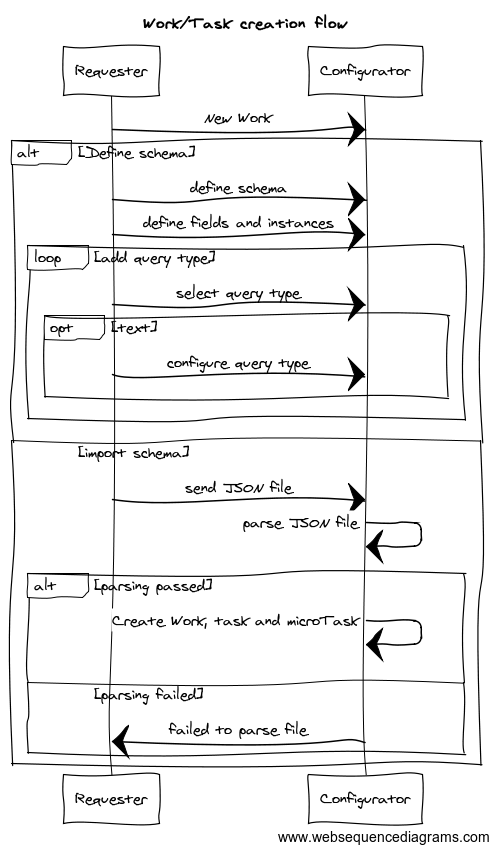
\includegraphics[width=0.65\columnwidth]{task-creation}
    \caption{Work/Task creation flow.}
    \label{fig:task-creation}
\end{figure}



\subsection{Task planning}
\begin{figure}[htb]
    \centering
    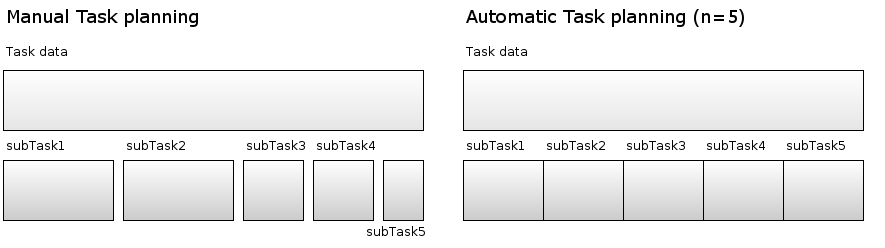
\includegraphics[width=\columnwidth]{planning}
    \caption{Manual Task planning vs Automatic Task planning.}
    \label{fig:auto-manual-planning}
\end{figure}
The planning of a Task involves the creation of subtasks with associated data
that need to be executed. The assignment can be performed automatically or
manually. The automatic plan assignment uses a simple subdivision based on the
number of instances to assign to each subTask.

As depicted in \autoref{fig:task-planning} manual planning involves the
\emph{Requester} interaction in order to create \textbf{subTasks}. After creating
the subTask the \emph{Requester} has to select the instances belonging to this
subTask. Eventually the \emph{Requester} is able to select and, if needed,
configure the type of the subTask, based on the task types of the parent Task.
\begin{figure}[htb]
    \centering
    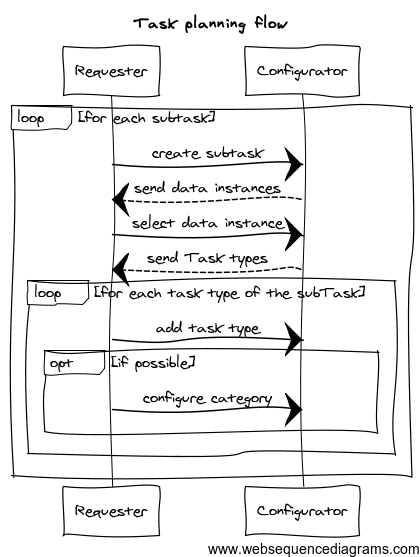
\includegraphics[width=0.65\columnwidth]{task-planning}
    \caption{Task planning flow.}
    \label{fig:task-planning}
\end{figure}



\subsection{Task execution}








